\documentclass{report}

\usepackage{fancyhdr}
\usepackage{fourier-orns}
\usepackage{hyperref}%% To refrence links / jumps
\usepackage{chngcntr} %% For some extra counters numberings
\usepackage[a4paper, right = 0.5in, left = 0.5in,top = 1in , bottom = 1in]{geometry}
\usepackage{etoolbox} %% Provides like a language for advanced customization
\usepackage{datetime} %% For dates of course
\usepackage{lastpage} %% provides pages numbers
\usepackage[sc]{titlesec} %% modify titles
\usepackage{enumerate}
\usepackage{cancel}
\usepackage{tikzsymbols}
\usepackage[dvipsnames]{xcolor}
\usepackage{import}
\usepackage{pdfpages} %% include other pdfs
\usepackage{transparent} %% Transparency
\usepackage{xcolor}  %% Colors
\usepackage[many]{tcolorbox}
\usepackage[framemethod=TikZ]{mdframed}
\usepackage{amsmath,amsfonts,amsthm,amssymb,mathtools}
\usepackage{tikz}
\usepackage{bookmark}
\usepackage{graphicx}
\usepackage{mathpazo}

\usepackage{fontawesome5}

\linespread{1.5}


\titleformat{\chapter}[display]   
{\fontfamily{ppl}\selectfont\huge\color{YellowOrange!80!orange}} % Font style and size 
{\raggedleft\color{purple}\fontsize{70}{0pt}\selectfont\thechapter}   
{-1.5cm}    			                          % Space between the chapter number and title
{
	\begin{tikzpicture}[overlay]
		\node[anchor = west,yshift = 0.2cm,xshift = -1cm] {\fontsize{90}{20} $\int_{}^{} $};
		\node[yshift = 4cm, xshift = 17cm]   {\includegraphics[width = 4cm]{preview0}};
	\end{tikzpicture}
\hspace{1cm}\Huge\raggedright\MakeUppercase}

\titleformat{\section}[block]
{
\fontfamily{ppl}\selectfont\huge\color{YellowOrange!80!orange}
}
{
\color{purple}\fontsize{20}{0pt}\selectfont\thesection 
}
{0cm}
{
	\begin{tikzpicture}[overlay]
		\node[anchor = west,yshift = 0.2cm,xshift = -0.4cm, circle = 1pt] {};
	\end{tikzpicture}
}

\titlespacing*{\section}{0pt}{0.7cm}{1.5cm}


\newcommand{\divider}
{
	\begin{center}
	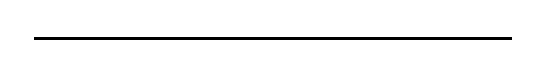
\begin{tikzpicture}
		\draw[thick, black] (0.25*\textwidth, 0) -- (0.75*\textwidth, 0);
		\node[rotate = 360 - 90, xshift = -0.6pt, yshift = 1pt] at (0.25*\textwidth,0){\decotwo};
		\node[rotate = 90, xshift = -0.6pt, yshift = 1pt] at (0.75*\textwidth,0){\decotwo};
	\end{tikzpicture}
	\end{center}
}

\pagestyle{fancy}

\newcommand{\lecday}[1][]
{
    \def\datee{#1}
    \fancyhead[L]{\datee}
}



\newcommand{\signature}
{
	\begin{tikzpicture}[remember picture,overlay]
		\node[fill = YellowOrange!20!white] at ([yshift = 1cm, xshift = -3cm]current page.south east) {\fontsize{10pt}{0pt}{\itshape Kara.$\mathcal{A}$}};
	\end{tikzpicture}
}

\AddToHook{shipout/background}{
  \begin{tikzpicture}[remember picture, overlay]
	  \node[] at ([yshift = 1.5cm,xshift = \textwidth /2 + 0.9cm]current page.south west) {\includegraphics[width = 0.5cm]{preview3}};
	  \node[] at ([yshift = 1.5cm,xshift = - \textwidth /2 - 0.9cm]current page.south east) {\includegraphics[width = 0.5cm]{preview4}};
  \end{tikzpicture}
}



\newtcolorbox[auto counter, number within = section]{remark}[1][]
{
       		title = Remark #1,
		enhanced,
		boxrule = 0pt,
		colback = white,
		breakable,
		arc = 4pt,
		colbacktitle = cyan,
		colback = cyan!5!white,
		segmentation style =
		{
			solid,cyan,thick,
		},
		attach boxed title to top left =
		{
			xshift = 0cm,
		},
		boxed title style =
		{
			boxrule = 0pt,
			sharp corners,
			drop fuzzy shadow = {cyan},
		},
		drop fuzzy shadow = {cyan!80!black},
}

\newtcolorbox[auto counter, number within = section]{theorem}[1][]
{                                      
		title = Theorem \thetcbcounter : #1,
		enhanced, 
		boxrule = 0pt,
		colback = white,
		breakable,
		arc = 4pt,
		colbacktitle = purple,
		colback = purple!5!white,
		segmentation style = 
		{
			solid, purple,thick,
		},
		attach boxed title to top left = 
		{
			xshift = 0cm, 
		},
		boxed title style = 
		{
			boxrule = 0pt,
			sharp corners,
			drop fuzzy shadow = {purple},
		},
		drop fuzzy shadow = {purple!80!black},
}

\newtcolorbox[auto counter, number within = section]{definition}[1][]
{                                      
		title = Definition \thetcbcounter : #1,
		enhanced, 
		boxrule = 0pt,
		colback = white,
		arc = 4pt,
		breakable,
		colbacktitle = YellowOrange!80!black,
		segmentation style = 
		{
			solid, YellowOrange,thick,
		},
		attach boxed title to top left = 
		{
			xshift = 0cm, 
		},
		colback = YellowOrange!5!white,
		boxed title style = 
		{
			boxrule = 0pt,
			sharp corners,
			drop fuzzy shadow = {YellowOrange!80!orange},
		},
		drop fuzzy shadow = {YellowOrange!80!black},
}

\newtcolorbox[auto counter, number within = section]{corollary}[1][]
{                                      
		title = corollary \thetcbcounter : #1,
		enhanced, 
		boxrule = 0pt,
		colback = white,
		arc = 4pt,
		breakable,
		colbacktitle = YellowOrange!80!black,
		segmentation style = 
		{
			solid, YellowOrange,thick,
		},
		attach boxed title to top left = 
		{
			xshift = 0cm, 
		},
		colback = YellowOrange!5!white,
		boxed title style = 
		{
			boxrule = 0pt,
			sharp corners,
			drop fuzzy shadow = {YellowOrange!80!orange},
		},
		drop fuzzy shadow = {YellowOrange!80!black},
}


\newtcolorbox{example}[1][]
{                                      
		title = Example,
		enhanced, 
		boxrule = 0pt,
		colback = white,
		arc = 4pt,
		segmentation style = 
		{
			solid, SpringGreen,thick,
		},
		breakable,
		colback = SpringGreen!5!white,
		colbacktitle = SpringGreen!80!black,
		attach boxed title to top left = 
		{
			xshift = 0cm, 
		},
		boxed title style = 
		{
			boxrule = 0pt,
			sharp corners,
			drop fuzzy shadow = {SpringGreen!80!orange},
		},
		drop fuzzy shadow = {SpringGreen!80!black},
}


\newcommand{\integral}[4]{\int\limits_{#1}^{#2} #4 d#3}
\newcommand{\limit}[3]{\lim\limits_{#1 \rightarrow #2} #3}
\newcommand{\strone}[2]{\left[ \begin{gathered}#1\\ #2\end{gathered} \right] }
\newcommand{\strtwo}[2]{\left\{ \begin{gathered}#1\\ #2\end{gathered} \right\} }
\newcommand{\strthree}[2]{\left\lfloor \begin{gathered}#1\\ #2\end{gathered} \right\rfloor }


\newcommand{\startbf}[1]{\text{\bfseries{#1}}}
\newcommand{\sett}[1]{\left\{ #1 \right\}}
\newcommand{\thesis}[1]{\left( #1 \right)}
\newcommand{\brkt}[1]{\left[ #1 \right]}
\newcommand{\floor}[1]{\left\lfloor #1 \right\rfloor}


\DeclareMathOperator{\img}{im} % Image
\DeclareMathOperator{\Img}{Im} % Image
\DeclareMathOperator{\coker}{coker} % Cokernel
\DeclareMathOperator{\Coker}{Coker} % Cokernel
\DeclareMathOperator{\Ker}{Ker} % Kernel
\DeclareMathOperator{\rank}{rank}
\DeclareMathOperator{\Spec}{Spec} % spectrum
\DeclareMathOperator{\Tr}{Tr} % trace
\DeclareMathOperator{\pr}{pr} % projection
\DeclareMathOperator{\ext}{ext} % extension
\DeclareMathOperator{\pred}{pred} % predecessor
\DeclareMathOperator{\dom}{dom} % domain
\DeclareMathOperator{\ran}{ran} % range
\DeclareMathOperator{\Hom}{Hom} % homomorphism
\DeclareMathOperator{\Mor}{Mor} % morphisms
\DeclareMathOperator{\End}{End} % endomorphism


\newcommand{\lm}{\ensuremath{\lambda}}
\newcommand{\eps}{\ensuremath{\epsilon}}
\newcommand{\veps}{\ensuremath{\varepsilon}}
\newcommand{\al}{\ensuremath{\alpha}}
\newcommand{\bb}{\ensuremath{\beta}}
\newcommand{\cc}{\ensuremath{\gamma}}
\newcommand{\dd}{\ensuremath{\delta}}
\newcommand{\DD}{\ensuremath{\Delta}}
\newcommand{\ff}{\ensuremath{\phi}}
\newcommand{\FF}{\ensuremath{\varphi}}

\newcommand{\RR}{\mathbb{R}}
\newcommand{\RO}{\mathcal{R}}
\newcommand{\EE}{\mathbb{E}}
\newcommand{\CC}{\mathbb{C}}
\newcommand{\RW}{\mathbb{R}^2}
\newcommand{\RT}{\mathbb{R}^3}
\newcommand{\RN}{\mathbb{R}^n}
\newcommand{\DS}{\mathcal{D}}

\newcommand{\KK}{\mathbb{K}}
\newcommand{\KW}{\mathbb{K}^2}
\newcommand{\KT}{\mathbb{K}^3}
\newcommand{\KN}{\mathbb{K}^n}

\newcommand{\NN}{\mathbb{N}}

\newcommand{\PS}{\mathcal{P}}
\newcommand{\AS}{\mathcal{E}}
\newcommand{\FS}{\mathcal{F}}
\newcommand{\LS}{\mathcal{L}}
\newcommand{\MS}{\mathcal{M}}


















\lecday[2025-05-15]

\begin{document}      

\section{The Geometric versions of the Hahn-Banach Theorem}      

\textbf{Lemma 02}
Let $(E,d)  $ be a metric
space and let $A $ and $B $ be two nonempty 
disjoint subsets of $E $ such that 
$A $ is closed and $B $ is compact
then we have $d(A,B) > 0$
\begin{proof}
Suppose for contradiction that $d(A,B) =0 $. Then by
the definition of $d(A,B):= \inf_{a \in  A, b \in B} d(a,b)$,
for all $n \in \NN$: there exists 
$a_{n} \in  A $ and $b_{n} \in  B $ such that, 
\[
d(a_{n}, b_{n})  <  \frac{1}{n}
\] 
since $B $ is compact, then we can extract a subsequence 
$(b_{n}) _{n \in  \NN} $ of $B $ a convergent
subsequence $\left( b_{n_{k}} \right)_{k \in \NN}$. 
let $b = \lim_{k \to \infty } b_{n_{k}} $, 
then for all $k \in \NN $, 
\begin{align*}
	d(a_{n_{k}}, b)  & \leq 
	d(a_{n_{k}}, b_{n_{k}})  + 
	d(b_{n_{k}}, b)  
	\\
			 & \leq 
	\frac{1}{n_{k}} + d(b_{n_{k}}, b) 
\end{align*}
hence, $\lim_{k \to \infty} d(a_{n_{k}}, b) = 0$, 
implying that the sequence $(a_{n_{k}})_{k \in  \NN}  $ of $A $ 
converges to $b $, then $b \in  \overline{A}= A $
since $A $ is closed, 
thus $b \in A \cap B = \emptyset  $, Contradiction hence
$d(A,B) > 0 $, as required.
\end{proof}
\begin{center}
\it Now we will prove the $1^{st} $ Geometric version of 
the Hahn-Banach theorem. \normalfont
\end{center}
\begin{align*}
 	C :&= A-B \\
	   &= 
	   \left\{ 
		   a-b, \in A, 
		   b \in  B
	   \right\}
\end{align*}
Since $A $ and $B $ are convex, then $C$ is 
convex, quick scratch proof, 
\divider
Let $c_1, c_2 \in  C $ and $E \in [0,1] $, does there
exists $ t c_1 + (1-t) c_2 \in C$,  
\begin{align*}
&\exists a_1 \in  A, b_1 \in  B \text{ such that } 
c_1 = a_1-b_1 \\
& \exists a_2 \in  A, b_2 \in  B \text{ such that }  
c_2 = a_2 - b_2
\end{align*}
thus 
\begin{align*}
	tc_1 + (1-t) c_2 &=
	t(a_1-b_1)  +
	 (1-t) (a_2-b_2)  \\
			 &= 
	\left( 
	\underbrace{
	ta_1 + (1-t) a_2
	}_{\in  A \text{ convex} } 
	\right) - 
	\left( 
		\underbrace{
		tb_1 + 
		(1-t) b_2
		}_{\in B 
		\text{ convex } } 
	\right) \in A - B = C
\end{align*} 
Thus $C $ is convex.
\divider
Since $A \neq \emptyset$ and $B \neq \emptyset  $  then 
$C \neq \emptyset  $, since $A $ and $B $ 
are disjoint then $0_{E} \notin C $, Next we remark 
that,
\[
C = \bigcup_{b \in B}^{}  
\left( 
	A - b
\right)
\]
\[
\begin{array}{cccc}
      \tau _{b} : &    E & \longrightarrow &  E\\
           &    x & \longmapsto     &  x+b\\ 
\end{array}
\]
For all $b \in B$, 
since $\tau _{b} $ is continuous 
and $A $ is open then $\tau ^{-1} _{b} (A) = A-b $  is open,
thus $C $ is a union of open
subsets of $E $ implying that $C $ is open in $E $.\\
By applying \textbf{Lemma 01} for the convex
subset $C $ of $E $ and for $x_0 = 0_{E} \notin C $, 
we find that there exist $f \in  E \backslash \left\{ 
	0_{E}
\right\} $ 
such that 
\[
f(x) <  f(0_{E})  = 0 \quad 
\quad 
\left( 
	\forall  x \in  C
\right)
\] 
writting $x = a-b \quad (a \in A, b \in B)  $, we conclude
that 
\[
f(a-b) <  0
\]
hence
\[
	f(a)  <  f(b)  \quad 
	\quad  
	\left( 
		\forall  a \in  A, \forall  b \in B 
	\right)
\] 
thus we get 
\[
\sup_{a \in A} f(a)  \leq 
f(b)  \quad \quad 
\left( 
	\forall  b \in  B
\right)
\] 
thus we get
\[
\sup_{ a \in A} 
f(a)  \leq 
\inf_{b \in B} f(b) 
\]
now consider $\al \in [\sup_{a \in A} f(a) , \inf_{b \in  B} f(b) ] $  
then we get for all $a \in  A $ an dfor all $b \in B $, 
\[
f(a) \leq \al \leq  f(b) 
\]
this completes the proof. 
\begin{proof}
Now we will prove the second geometric version of the Hahn-
Banach Theorem
\end{proof}
Since $A \cap B = \emptyset  $, and $A $ 
is closed and $B $ is compact then there exist by 
\textbf{Lemma 02} $d(A,B) > 0 $, fix $\veps  > 0 $ such that
\[
	\veps  < \frac{1}{2}
	d(A,B) 
\] 
now conisder
\begin{align*}
	A_{\veps } &=
	A + B_{E}(0_{E},\veps )  \\
	B_{\veps }&=
	B + B_{E}(0_{E},\veps ) 
\end{align*}
It's clear that $A _{\veps } $ and 
$B_{\veps } $ are non empty since $A,B$ and 
$B_{E}(0_{E}, \veps )  \neq  \emptyset  $. \\
Next, $A_{\veps } $ and $B_{\veps } $  are both convex
since they are sums of convex subsets, next 
$A_{\veps } $ and $B_{\veps } $ are disjoint, 
Indeed, suppose for contradiction that 
$A_{\veps } \cap B_{\veps }\neq  \emptyset  $, 
then there exist $x \in  E $ such that $x \in  A_{\veps }
\cap B_{\veps }$, then we can write $x $ as,
\[
x = a + u = b + v
\quad \quad (u,v\in  B_{E}(0_{E},1)\quad a,b \in  A,B)
\] 
Thus, 
\begin{align*}
	\| a-b \|  &=
	\| v-u \|  \\
		   & \leq 
		   \underbrace{
	\| v \| 
		   }_{ <  \veps }  + 
		   \underbrace{
	\| u \| 
		   }_{ <  \veps } \\
		  < 2 \veps  <  
		  d(A,B)  < 
		  \| a-b \| 
\end{align*}
hence $\| a-b \| <  \| a-b \|  $, which is a contradiction
thus $A_{\veps } \cap B_{\veps } = \emptyset  $, 
as claimed let us show that $A_{\veps } $ 
is open, then we can write 
\[
A_{\veps }= 
\bigcup_{ a \in  A}^{}  
\left( 
	a + B_{E}(0_{E}, \veps ) 
\right) = 
\bigcup_{ a \in  A}^{}  
B_{E}(a, \veps ) 
\] 
which is a union of open subsets of $E$, thus 
$A_{\veps } $ is open, now by applying the first 
geometric version of the Hahn-Banach for $A_{\veps } $ 
and $B_{\veps } $, we can find that there exists 
a functio in $E' \backslash \left\{ 0_{E '} \right\} $  and
there exists $\al \in  \RR  $  such that, 
\[
f(x) \leq \al \leq f(y)  \quad 
\quad 
\left( 
	\forall x \in  A_{\veps },
	\forall y \in B_{\veps }
\right)
\]
now we can write $x,y \in  A_{\veps },B_{\veps } $  like this, 
\begin{align*}
	x &= 
	a + \veps u , \quad \quad a \in  A, u \in 
	B_E(0_{E},1)  \\
	y &= b + \veps v, \quad \quad 
	b \in  B, v \in  B_{E}(0_{E},1) 
\end{align*}
we set, 
\begin{align*}
f(a) + \veps f(u)  \leq 
\al 
\leq f(b) + \veps f(v) 
\quad 
\quad 
\left( 
	\forall a,b \in A,B, 
	\forall u,v \in  B_{E}(0_{E},1) 
\right)
\end{align*}
Hence, 
\[
	f(a)  + \veps 
	\sup_{u \in  B_{E}(0_{E},1) }  
	f(u) \leq 
	\al \leq 
	f(b) + \veps 
	\inf_{v \in  B_{E}(0_{E},1) }  
	f(v) 
\]
But, 
\begin{align*}
	\sup_{u \in  B_{E}(0_{E},1) }  
	f(u) &=
	\sup_{u \in  B_{E}(0_{E},1) }  
	\| f(u)  \|  &= 
	f( (+/-)  u)  \\
		     &= \mid \mid \mid  f \mid \mid \mid 
\end{align*}
and we have, 
\begin{align*}
\inf_{u \in  B_{E}(0_{E,1}) }  
f(u)  &=
- \sup_{u \in  B_{E}(0_{E},1) }  
(-f(u) )  \\
      &= -\sup_{u \in  B_{E}(0_{E},1)f(-u)  }  \\
      &= - \mid \mid \mid f  \mid \mid \mid 
 \end{align*}
 hence, 
 \[
 f(a) + \veps 
 \mid \mid \mid  f \mid \mid \mid  \leq 
 \al \leq 
 f(b) - \veps \mid \mid \mid  f \mid \mid \mid   
 \quad \quad 
	\left( 
		\forall a,b \in A,B
	\right)
 \]
hence 
\[
f(a) <  \al <  f(b)  \quad \quad 
(\forall  a \in  A, b \in  B) 
\]
This completes the proof.
\newpage
\chapter{The Hilbert-Spaces}  
\section{Generalities}
\begin{definition}[(Real inner Product]
	Let $E $ be an $\RR  $-vector space, we call
	inner product on $E$ any 
	\it \textcolor{red}{Positive} 
	\textcolor{blue}{DefinitE} 
	\textcolor{green}{Symmetric} 
	\textcolor{yellow}{Billinear}
	\textcolor{purple}{Form}
	\normalfont
	on 
	$E$, that is any map,
	$ f :E^2   \longrightarrow \RR  $, 
	Satisfying the following properties:\\
	$\forall x,y,x_1, x_2, y_1, y_2 \in  E $, and for 
	all $\lm_1,\lm_2 \in  \RR  $:
	\begin{enumerate}[(i)]
		\item 
			\[
			f(\lm_1 x_1 + \lm_2 x_2, y)  =
		\lm_1f(x_1, y) + \lm_2 f(x_2, y) 
			\]
			\hfill
			( \textcolor{red}{Linearity with respect
			to $1 ^{st} $ argument})
		\item 
			\[
			f(x, \lm_1 y_1 + \lm_2 y_2)  =
			\lm_1 f(x, y_1)  + 
			\lm_2 f(x, y_2) 
			\]
			\hfill
			(\textcolor{blue}{Linearity with respect
			to $2 ^{nd} $ argument})
		\item The symmetry:
			\[
			\forall x,y \in  E : \quad 
			f(x,y) = f(y,x) 
			\]
		\item Positive definitness: 
			\begin{align*}
			\begin{cases}
			\forall x \in  E :
			\quad f(x,x) \geq 0 
			\quad \quad 
			\text{ \textcolor{red}{Positive semi-definitness }}  \\
			\forall x \in  E: 
			\quad f(x,x) = 0 \implies 
			x= 0_{E} 
			\quad \quad 
			\text{ \textcolor{red}{Definite}} 
			\end{cases}
			\end{align*}
			which is equivallent to, 
			\[
			\forall x \in  E \backslash 
			\left\{ 0_{E} \right\} : 
			\quad f(x,x) > 0
			\]
	\end{enumerate}
\end{definition}
\begin{definition}[(Complex inner product)]
	Let $E $ be a $\CC  $-vector space, we call
	inner product on $E $ any positive definit
	hermitian form on $E$, that is any map 
	$ f : E^2  \longrightarrow \CC  $, satisfying the following
	properities: 
	\begin{enumerate}[(i)]
	\item Semi-linearity in the first argument: \it (sesqui = 1.5 linear)
		\normalfont
		\[
		\forall x_1,x_2,y \in E, 
		\forall \lm_1, \lm_2 \in \CC
		\]
		we have, 
		\[
		f(\lm_1 x_1 + \lm_2x_2, y)  =
		\overline{\lm_1} 
		f(x_1, y)  + 
		\overline{\lm_2}
		f(x_2, y) 
		\]
	\item Linearity in the second argument:
		\[
		\forall x,y_1,y_2 \in  E, 
		\forall \lm_1, \lm_2 \in \CC :
		\] 
		in other words, 
		\[
		f(x, \lm_1 y_1 + \lm_2 y_2)  = 
		\lm_1 f(x, y_1) + \lm_2 f(x,y_2) 
		\]
	\item Hermitian Symmetry: 
		\[
		\forall x,y \in  E: 
		\overline{f(x,y) }= 
		f(y,x)  
		\]
		which implies, 
		\[
		\forall x \in  E: \quad 
		\overline{f(x,x) } = f(x,x)  \implies 
		\forall x \in  E: f(x,x) \in \RR 
		\] 
	\item Positive definiteness:
	\begin{align*}
	\begin{cases}
	\forall x \in  E: 
	\quad f(x,x) \geq 0 \quad \quad 
	\text{ \textcolor{red}{Positive semi-definitness}}  \\
	\forall x \in  E: \quad 
	f(x,x) = 0 \implies 
	x = 0_{E} \quad 
	\quad \text{ \textcolor{red}{Definiteness}} 
	\end{cases}
	\end{align*}
	which is equivalent to,
	\[
	\forall x \in  E \backslash \left\{ 0_{E} \right\} : 
	f(x,x)  > 0
	\]
	\end{enumerate}
\end{definition}
\divider
\textbf{NB : } ~ \it 
The standard notation of an inner product (real or complex) is: 
\[
\left\langle . , . \right\rangle 
\]
\divider
\begin{center}
	\textbf{Examples} \it 
	\fbox{
	\lefthand ~  in finite-dimensional vector spaces
	}
\end{center}
Let $n \in  \NN $ be fixed, 
\begin{enumerate}
\item The standard inner product $\RR ^n  $  (seen as an 
	$\RR$-vector space) is defined by:
	\[
	\forall  x= 
	\begin{pmatrix}
		x_1 \\
		x_2 \\
		\vdots  \\
		x_{n} \\
	\end{pmatrix} , y=
	\begin{pmatrix}
		x_1 \\
		x_2 \\
		\vdots  \\
		x_{n} \\
	\end{pmatrix} 
	\in  \RR ^n 
	: \quad \left\langle x,y \right\rangle _{us} := 
	x_1 y_1 + x_2 y_2 +  \hdots + x_n y_n 
	\]
\item The standard inner product of $\CC  $ (seen as $\CC  $-vector space)  
	is defined by, 
	\[
	\forall  z= 
	\begin{pmatrix}
		z_1 \\
		z_2 \\
		\vdots  \\
		z_{n} \\
	\end{pmatrix} , w=
	\begin{pmatrix}
		w_1 \\
		w_2 \\
		\vdots  \\
		w_{n} \\
	\end{pmatrix} 
	\in  \CC  ^n  : 
	\left\langle 
		z,w 
	\right\rangle _{us} = 
	\overline{z_1}w_1 + 
	\overline{z_2}w_2 + \hdots +
	\overline{z_n }w_n 
	\]  
	note that, 
	\[
		\overline{\left\langle z,w \right\rangle } =
		\left\langle z,w \right\rangle 
	\] 
\end{enumerate}
\begin{center}
	\textbf{Examples} \it 
	\fbox{
	\lefthand ~ in infinite-dimensional vector spaces
	}
\end{center}
\begin{enumerate}[(1)]
\item  Let $a,b \in  \RR  $  such that $a <  b $ Consider the 
	$\RR  $-vector space  
	$\mathcal{C}^{0} ([a,b], \RR ) $ of continuous real-valued
	functions on $[a,b]  $. \\
	The Properties of the \textcolor{blue}{Riemann} Integrals 
	easily show that the map defined by: 
	\[
	\begin{array}{cccc}
	      \left\langle \cdot .\cdot  \right\rangle  : &  
	      \mathcal{C} ^{0}([a,b],\RR ) \mathcal{C} ^{0}([a,b],\RR ) 
		  & \longrightarrow &  \RR \\
	
	           &(f,g)     & \longmapsto     &  
		   \int_{a}^{b} 
		   f(t) g(t) dt
		   \\
	\end{array}
	\]
	is an inner product on $\mathcal{C} ^{0}([a,b],\RR )  $  
\item Let $a,b \in  \RR  $ such that $a < b $. Consider the 
	$\CC  $-vector space 
	$\mathcal{C} ^{0}([a,b],\CC ) $  of continuous
	complex-valued functions on $[a,b] $, Using the properties
	of the \textcolor{blue}{Riemann} integrals  
	\[
	\begin{array}{cccc}
	      \left\langle \cdot .\cdot  \right\rangle  : &  
	      \mathcal{C} ^{0}([a,b],\CC  ) \mathcal{C} ^{0}([a,b],\CC  ) 
		  & \longrightarrow &  \CC  \\
	
	           &(f,g)     & \longmapsto     &   
		   \left\langle f,g \right\rangle 
		   \\
	\end{array}
	\]
	is an inner product on $\mathcal{C} ^{0}
	([a,b],\CC)$  
	\divider
	\begin{align*}
		\overline{\left\langle f,g \right\rangle } 
		&=
		\overline{
	\int_{a}^{b} 
	\overline{f(t) }g(t) dt 
		}
\\
	   &= 
	   \int_{a}^{b} 
	   \overline{\overline{f(t) }} 
	   \overline{g(t) } dt \\
	   &=
	   \int_{a}^{b} 
	   \overline{g(t) } 
	   f(t) dt = 
	   \left\langle g,f \right\rangle 
	   \\
	\end{align*}
\end{enumerate}
\normalfont
\newpage
\section{The norm associated to an inner product }
\begin{definition}[]
Let $\KK = \RR $  or $\CC  $ and let $E $ be a $\KK $-vector space,
equipped with an inner product $\left\langle \cdot , \cdot  \right\rangle  $.\\
We define the 
\underline{ norm associated to }
$\left\langle \cdot , \cdot  \right\rangle  $ as the map: 
\[
\begin{array}{cccc}
	\| . \|  : &  E  & \longrightarrow & [0, \infty ) \\

           &    x& \longmapsto     &  \| x \|  =  
	   \sqrt{\left\langle x,x \right\rangle } \\ 
\end{array}
\]
since $\left\langle \cdot ,\cdot  \right\rangle  $ 
is positive definite then 
$\| \cdot  \|  $ is well-defined and 
\[
\left( 
	\forall  x \in  E: \quad 
	\| x \| = 0 \implies 
	x = 0_{E}
\right)
\]
Next, we have that for all $x \in  E $, and for all $\lm \in  \KK $: 
\begin{align*}
	\| \lm x \|  &=
	\sqrt{\left\langle 
			\lm x, \lm x
	\right\rangle }  \\
	&= \sqrt{
		\overline{\lm } \lm 
		\left\langle 
			x, x
		\right\rangle 
	} \quad \quad 
	\quad 
	\text{
		\textcolor{red}{
		$\KK = \CC  $ for example
		}
	} 
	\\
	&= \sqrt{ \left| \lm \right|^2  \| x \| ^2 }  =
	\left| \lm \right| \| x \| 
\end{align*}
We will see later that $\| \cdot  \|  $, also satisfies the triangle
inequality: 
\[
\| x+y \|  \leq \| x \| + \| y \| \quad 
\quad 
\left( 
	\forall x,y \in  E
\right)
\]
So $\| . \|  $  is realy a norm on $E $ 
\end{definition}
\section{The Cauchy-Schwarz Inequality}
\begin{theorem}[]
Let $\KK = \RR  $ or $\CC  $ and be a $\KK $-vector space equipped
with an inner product 
$\left\langle \cdot ,\cdot  \right\rangle  $. Let also 
$\| \cdot  \|  $ denote the norm associated to 
$\left\langle \cdot  , \cdot  \right\rangle  $, 
then we have for all $x,y \in E $ : 
\[
	\fbox{
		$  
		\left| 
		\left\langle x, y \right\rangle    
		\right|
		\leq \| x \| \cdot  \| y \| $  
	}
\]
Its the \textcolor{blue}{Cauchy Schwarz}, In addition this 
inequality becomes an equality \underline{ if and only if } 
$x $ and $y $ are collinear.
\end{theorem}
\end{document}
